\documentclass[11pt]{article}
\usepackage[a4paper, left=2cm, right=2cm, top=2cm, bottom=2cm]{geometry}
\usepackage{graphicx}
\usepackage{natbib}
\usepackage[toc,page]{appendix}
\usepackage{float}
\usepackage{amsmath,amssymb}
\usepackage{varwidth}
\usepackage{xcolor}
\usepackage{url}
\usepackage[font=footnotesize]{caption}
\usepackage{subfig}
\usepackage{hyperref}
\usepackage{cleveref}

% Comment if need more space
\usepackage[nodisplayskipstretch]{setspace} \doublespacing\setlength{\jot}{7pt}

% Indentation for first paragraph
\usepackage{indentfirst}
\setlength{\parindent}{1.5em}

% Put highlight on equation
\usepackage{xcolor}
\usepackage{soul}
\newcommand{\mathcolorbox}[2]{\colorbox{#1}{$\displaystyle #2$}}
\definecolor{mygray}{gray}{0.85}

\newcommand{\grad}{\operatorname{grad}}
\newcommand{\dive}{\operatorname{div}}
\DeclareMathOperator{\g}{g}
\DeclareMathOperator{\G}{G}
\DeclareMathOperator{\T}{T}
\DeclareMathOperator{\R}{R}


\begin{document}

% Cover Page
\begin{titlepage}


    \begin{flushleft}
        \vspace{-2.2cm}
        
\includegraphics[width=4cm]{Images/college_logo.jpg}
    \end{flushleft}
    
    \vspace{7cm}
    
    \centering
    {\huge\textbf{Spherical Characteristic Numerical Relativity} \par}
    
    \vspace{5cm}
   
    {\large First Cycle Integrated Project in Engineering Physics\par}
    \vspace{0.5cm}
    {\large Scientific Project\par}
    \vspace{3cm}
    {\large Joana Yao\par}
    \vspace{0.5cm}
    {\large Orientation: David Hilditch\par}
    
    \vfill
    
    {\large 2024\par}
\end{titlepage}

% Abstract
\noindent
\hrulefill% Upper horizontal line
\begin{center}
    \section*{Abstract}

\end{center}
\hrulefill% Lower horizontal line
\vspace{0.5cm}

\section{Introduction}

This project aims to make a programme to deduce and solve the Einstein-scalar Equations in double null coordinates with spherical symmetry with initial conditions in a null slice and replicate the result in the paper \textcolor{red}{write reference}

and see if it collapses or not and blabla I probably cant even do this

The ones who worked in this are blabla and bla

Advantage of null coordinates: Before it was done with mesh refinement but with these coordinates, the resolution gets better by itself

We also check the correctness of the numerical methods implemented

The plots throughout this report were done using Matplotlib~\cite{Matplotlib}.

\section{Formulation of Null Initial Value Problem}\label{sec: Formulation}

In general, a spherically symmetric metric in null coordinates is
\begin{align}
    ds^2 = 2\g_{uv}dudv + r^2d\Omega^2\, , \label{eq: double null metric}
\end{align}
where $u$ and $v$ are the null coordinates $d\Omega^2 = d\theta^2+\sin^2\phi\,d\phi^2$ is the metric for a 2-sphere, and $r$ is the usual radial coordinate, which will be regarded as a function of $u$ and $v$. The coordinates are defined as follows: $u$ is the proper time of an observer at the origin (that is, at $r=0$) and is constant on outgoing light rays and $u$ = 0 is the initial data surface; the coordinate $v$ is constant on ingoing light rays and is equal to two times the usual area coordinate $r$ on the initial data surface.

The Einstein Equations (without cosmological constant) are
\begin{gather}
    G_{\mu\nu}=8\pi\T_{\mu\nu} \, .
\end{gather}
where $\G_{\mu\nu}$ is the Einstein tensor and $\T_{\mu\nu}$ is the energy-momentum tensor.
For a massless scalar field, the energy-momentum tensor is $T_{\mu\nu}=\partial_\mu\Phi\partial_\nu\Phi-\frac{1}{2}\g_{\mu\nu}g^{\alpha\beta}\partial_\alpha\Phi\partial_\beta\Phi $, so these equations become
\begin{align}
    \R_{\mu\nu}=8\pi\partial_\mu\Phi\partial_\nu\Phi 
    \label{eq: Einstein eqs}
\end{align}
where $\R_{\mu\nu}$ is the Ricci tensor and $\Phi$ is the scalar field. Both $\G_{\mu\nu}$ and $\R_{\mu\nu}$ can be computed from the metric $\g_{\mu\nu}\,$. \textcolor{red}{Put def of ricci tensor, maybe on annex}

We now introduce some notation used from here on. For any function f, we define
\begin{gather}
    f' \equiv \frac{\partial f}{\partial v} \, ,\\
    \dot f \equiv \frac{\partial f}{\partial u} \, , \\
    \Bar{f} \equiv \frac{1}{r}\int_0^r f dr = \frac{1}{r}\int_{r=0}^v f(u,\tilde{v}) r'(u,\tilde{v}) d\tilde{v}\, .\label{eq: bar definition}
\end{gather}
where the $r=0$ in the integral limit means ``$v$ such that $r(u,v)=0$''.

Now, defining $h$ such that $\bar h = \Phi$, we can use the Einstein equations to write the metric as a function of $h$ and $r$. We also define some useful quantities
\begin{gather}
    q \equiv r^{-1}(h-\bar h)^2 \, ,\\
    g \equiv \exp{(4\pi r \bar q)} \, .
\end{gather}
Then the $(\theta,\theta)$ equation in~\eqref{eq: Einstein eqs} gives
\begin{align}
    1- 2\frac{\partial_v r\partial_u r + r \partial_u\partial_v r}{\g_{uv}} = 0 \Leftrightarrow
    \g_{uv} = 2 \partial_v (r \partial_u r) \Leftrightarrow 
    \frac{1}{2r}\int_{r=0}^v \g_{uv}(u,\tilde{v}) d\tilde{v} = \dot r \, , \label{eq: g_uv rdot}
\end{align}
and the $(v,v)$ equation yields
\begin{gather}
    \frac{2 \partial_v \g_{uv}\partial_v r - 2\g_{uv}\partial_v^2 r}{\g_{uv}r} = 8\pi(\partial_v \bar h)^2 \Leftrightarrow \frac{\partial_v \g_{uv}}{\g_{uv}} = \frac{4\pi r (\partial_v \bar h)^2 + \partial_v^2 r}{\partial_v r} \,\notag\\
    \Leftrightarrow \frac{\g_{uv}}{\g_{uv}(r=0)} = \exp{\left[\int_{r=0}^v \frac{4\pi r (\partial_v \bar h)^2}{\partial_v r} + \partial_v \ln{\partial_v r}\,d\tilde{v}\right]} .\label{eq: (v,v) equation}
\end{gather}
Using some arithmetric and the definition in equation~\eqref{eq: bar definition} we obtain
\begin{align}
    \partial_v \Bar{h} = \frac{r'}{r}(h-\Bar{h}) \, , \label{eq: partial_v of hbar}
\end{align}
so equation~\eqref{eq: (v,v) equation} becomes 
\begin{gather}
    \g_{uv} = \g_{uv}(r=0)\exp{\left[4\pi r \bar{q} + \ln{(r')} - \ln{(r'(r=0))}\right]} = \frac{\g_{uv}(r=0)}{r'(r=0)} r'g \label{eq: g_uv almost}
    %\\    \g_{uv}= - r'g \label{eq: g_uv}
\end{gather}

Substituting expression~\eqref{eq: g_uv almost} in equation~\eqref{eq: g_uv rdot} we get
\begin{align}
    %\mathcolorbox{mygray}{\dot r = - \frac{1}{2} \bar{g}}
    \dot r = \frac{1}{2}\frac{g_{uv}(r=0)}{r'(r=0)}\bar{g}\, \Rightarrow \dot r(r=0) = \frac{1}{2}\frac{g_{uv}(r=0)}{r'(r=0)}\, \Rightarrow \dot r(r=0) = \frac{1}{4}g_{uv}(r=0) . 
    \label{eq: rdot r=0}
\end{align}
where in the last step we chose $r'(r=0) = 1/2\,$, giving $\g_{uv}(r=0) = -1/2$ as a result of the definition of $u$ as the proper time at $r=0\,$. 

To understand why $\g_{uv}(r=0) = -1/2\,$, we first use coordinates $(u,r,\theta,\phi)$ instead of $(u,v,\theta,\phi)$. In these coordinates, an observer at the origin ($r=0$) has a worldline $x(\lambda) = (u(\lambda),0,\theta(\lambda),\phi(\lambda))$. Moreover, using $dr = r' dv + \dot r du\,$, the metric~\eqref{eq: double null metric} becomes
\begin{align*}
    ds^2 = \frac{2}{r'}\g_{uv}dudr - 2\frac{\dot r}{r'}\g_{uv}du^2 + r^2 d\Omega^2
\end{align*}
Choosing affine parameter $\lambda=u$, we get $\dot x = (1,0,\dot\theta,\dot\phi)$. So the proper time at the origin is
\begin{gather*}
    \tau = \int_0^u \sqrt{-\tilde\g_{\mu\nu}\dot x^\mu \dot x^\nu} d\lambda = u\sqrt{-\tilde\g_{uu}} \, .
\end{gather*}
For u to be the proper time, we need $\tilde\g_{uu}=-1$ at $r=0\,$. That is,
\begin{align*}
    -1 = - 2 \frac{\dot r(r=0)}{r'(r=0)}\g_{uv}(r=0) \Leftrightarrow 
    1 = 4(\g_{uv}(r=0))^2
    \Leftrightarrow
    \g_{uv}(r=0) = -\frac{1}{2}
\end{align*}
where in the second step we used~\eqref{eq: rdot r=0} and in the last step we used the fact we choose that both $u$ and $v$ point to the future.

Thus the double null coordinates becomes
\begin{gather}
ds^2 = -2\,g\,r'\,dudv + r^2\,d\Omega^2
\end{gather}
and we get
\begin{gather}
    \boxed{\,\dot r = \frac{1}{2}\,\bar g\,}\, . \label{eq: rdot}
\end{gather}

Due to Bianchi identities $\nabla_\nu\G^{\mu\nu} = 0$, we have $\nabla_\nu\T^{\mu\nu} = 0$ which is equivalent to $\partial^\mu\bar{h}\,\square\bar{h}=0\,$,
and so one of the Einstein equations can be substituted by $\square \bar{h}= 0$, resulting in
\begin{gather*}
    \square \bar{h}= 0 \Leftrightarrow \frac{1}{\sqrt{-\g_\mu^{\;\;\mu}}\,\partial_\alpha(\sqrt{-\g_\mu^{\;\;\mu}}\,\partial^\alpha\bar{h})} = 0 \Leftrightarrow \partial_v\bar{h}\partial_u r + \partial_v r \partial_u\bar{h} + r\partial_u\partial_v\bar{h} = 0\\
    \Leftrightarrow \partial_u(\partial_v r(h-\bar{h})) + \partial_v r \partial_u \bar{h} = 0\Leftrightarrow (\partial_u\partial_v r)(h-\bar{h}) + \partial_v r\partial_u h = 0\\
    \Leftrightarrow \partial_v(-\frac{1}{2} \bar{g})(h-\bar{h}) + r'\dot h=0 \Leftrightarrow \dot h = \frac{1}{2r'}(\partial_v \bar g)(h-\bar{h})\, .
\end{gather*}
Now, using the result in equation~\eqref{eq: partial_v of hbar}, we obtain
\begin{align}
    %\mathcolorbox{mygray}{\dot h = \frac{1}{2r}(g - \bar g)(h-\bar{h})\, .}
    \boxed{\,\dot h = \frac{1}{2r}(g - \bar g)(h-\bar{h})\,}\, .
    \label{eq: hdot}
\end{align}

Equations~\eqref{eq: rdot} and~\eqref{eq: hdot} are thus the evolution equations for $r$ and $h$.

\section{Numerical Method}

We represent $h$ and other quantities on a grid at fixed values of $v$ and numerically evolve in the coordinate $u$.
We first start with initial data for the Einstein-Scalar equations which is just the value of $h$ for $u=0$ and, as mentioned in section~\ref{sec: Formulation}, $r=v/2$ at $u=0$. Using this data, we calculate the quantities $\bar h$, $q$, $g$ and $\bar g$ by evaluating the integrals using numerical integration. Using the evolution equations for $\dot h$ and $\dot r$, we evolve $h$ and $r$ forward one time step. The time evolution was done with fourth order Runge-Kutta method.

However, one source of innacuracy is division by r when evaluating these quantities, which is more problematic when near $r=0$. To solve this, we first expand $h$ in Taylor series
\begin{gather}
    h = h_0 + h_1\, r + O(r^2)\, \,,\label{eq: h expansion}
\end{gather}
so the Taylor expansion for $\bar h$, $q$, $g$ and $\bar g$ becomes
\begin{gather}
    \bar h = h_0 + h_1\, \frac{r}{2} + O(r^2) = h - h_1 \,\frac{r}{2} + O(r^2)\,\,,\label{eq: hbar expansion}\\
    q = \frac{1}{4}\, h_1^2 \,r\,\,,\label{eq: q expansion}\\
    g = 1 + \frac{\pi}{2}\, h_1^2\, r^2\,\,,\label{eq: g expansion}\\
    \bar g = 1 + \frac{\pi}{6} \, h_1^2\, r^2\,\,.\label{eq: gbar expansion}
\end{gather}

Then we fit the first four values of $h$ to a straight line (using simple linear regression) and find the values for $h_0$ and $h_1$. We next evaluate $\bar h$, $q$, $g$ and $\bar g$ using equations (\ref{eq: hbar expansion} $-$~\ref{eq: gbar expansion}) for the first three values of $r$. Numerical integration is then used for all other values of $r$.

\subsection{Convergence of Numerical Methods}

In order to check the correctness of the numerical methods, convergence tests were used. As numerical results are nothing more than approximations of the analytical solutions, we need some way to measure the errors in the approximations. Moreover, we expect these errors to get smaller as the resolution is increased.
The approximation can be interpreted as a continuum function that can be expanded as a porwer series of the discretization parameter $\Delta$
\begin{gather}
    S_\Delta (t,x) = S(t,x) + \sum_{i=1}^{\infty}\Delta\,e_i(t,x) \, ,
\end{gather}
where S(t,x) is the analytical solution, and $e_i(t,x)$ are error functions at different orders in $\Delta$. As an example, we expect $e_1 \neq 0$ for a first order accurate approximation, and for a second order accurate approximation we expect $e_1=0$ and $e_2\neq0\,$. 

There exist two types of convergence: pointwise convergence or norm convergence. To do the tests, we calculate the solution at three different resolutions $\Delta_1 > \Delta_2 > \Delta_3$

\subsubsection*{Pointwise Convergence}



\subsubsection*{Norm Convergence}


\subsection{Simpson's Rule for Unequally Spaced Data}

In this project, we used Simpson's rule for irregularly spaced data to integrate. This method approximates every three points to a parabolic function, and so the integral in an interval $[a,b]$ with an even number $N$ of sub-intervals $h_k$ is given by
\begin{align}
    \int_a^b f(x) dx\approx\sum_{i=0}^{N/2-1}\frac{h_{2i}+h_{2i+1}}{6}\left[\left(2-\frac{h_{2i+1}}{h_{2i}}\right)f_{2i}+\frac{(h_{2i}+h_{2i+1})^2}{h_{2i}h_{2i+1}}f_{2i+1}+\left(2-\frac{h_{2i}}{h_{2i+1}}\right)f_{2i+2}\right] \, .
    \label{eq: simpson rule}
\end{align}

In the case the number of slices $N$ is odd, we use the formula~\eqref{eq: simpson rule} up until the second to last interval and then add the quantity
\begin{align}
    &\alpha f_N + \beta f_{N-1} - \eta f_{N-2}\, ,
\end{align}
where
\begin{gather}
    \begin{aligned}
        &\alpha=\frac{2h_{N-1}^2+3h_{N-1}h_{N-2}}{6(h_{N-2}+h_{N-1})}\, ,\\
        &\beta=\frac{h_{N-1}^2+3h_{N-1}h_{N-2}}{6h_{N-2}}\, ,\\
        &\eta=\frac{h_{N-1}^3}{6h_{N-2}(h_{N-2}+h_{N-1})}\, .
    \end{aligned}
\end{gather}

To test this algorithm, we used as integrand a Gaussian distribution with $\sigma=1$ and $\mu=0$, integrating it between $-4.5$ and $4.5$ using an equally spaced grid, resulting in the figure~\ref{fig:gauss_integral}. We can see the result looks reasonably satisfactory.

\begin{figure}[H]
    \centering
    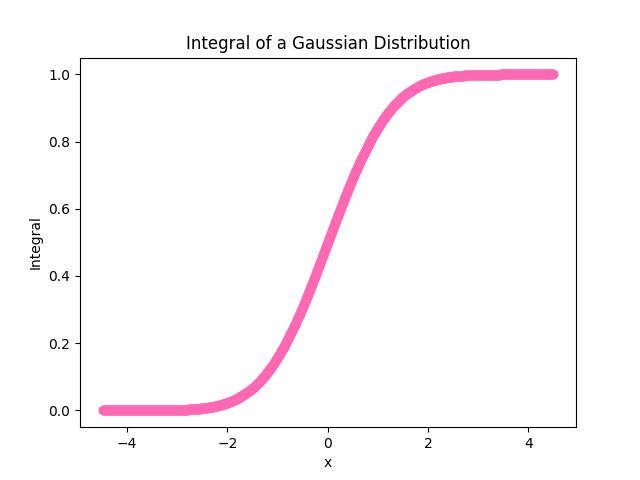
\includegraphics[width=0.5\linewidth]{Images/gauss_integral.png}
    \caption{Integral of a Gaussian distribution with $\sigma=1$ and $\mu=0$ using Simpson's Rule and with step $h=0.01$}\label{fig:gauss_integral}
\end{figure}

To conclude the result is indeed satisfactory, we check the pointwise convergence of the Simpson Rule. For that, we need to differentiate the points where the integral is calculated with an even number of slices or with an odd number of slices because the method is different for each of them.

\begin{figure}[H]
    \centering
    \subfloat[Odd slices]{\includegraphics[width= 0.5\linewidth]{Images/Simp_conv_odd.png}}
    \subfloat[Even slices]{\includegraphics[width= 0.5\linewidth]{Images/Simp_conv_even.png}}
    \caption{Comparison of the difference between the obtained integral with low (step $h = 0.09$) and middle (step $h = 0.03$) resolution, and of the different between the obtained integral with middle (step $h = 0.03$) and high (step $h = 0.01$), where the later one is scaled by $3^4$. The line and point plots were done to facilitate visualisation}\label{fig:simp_conv}
\end{figure}

Thus, we see that this Simpson's rule has a convergence of fourth order for even and odd number of slices.

\subsection{Trapezoidal Rule}

The trapezoidal rule consists of approximating every two points to a straight line and so the integral is given by
\begin{gather}
    \int_a^b f(x)dx \approx \sum_{i=0}^{n} \frac{1}{2}(f(x_i)+f(x_{i+1}))(x_{i+1}-x_i) \, .
\end{gather}

Its 

\subsection{Fourth Order Runge-Kutta (RK)}

In order to evolve the differential equations, fourth order RK method was used. The method is as follows. Let the initial-value problem be
\begin{gather}
    \frac{dy}{dt} = f(t,y)\quad, \quad y(t_0)=y_0 \quad .
\end{gather}
The evolution of $y$ for a time step $\Delta t$ combines information from four different (intermediate) steps and is then given by
\begin{gather}
    \begin{aligned}
        &K_1 = f(t_n, y_n)\, ,\\
        &K_2 = f(t_n + \frac{\Delta t}{2}, y_n + \Delta t\, \frac{K_1}{2})\,,\\
        &K_3 = f(t_n + \frac{\Delta t}{2}, y_n + \Delta t\, \frac{K_2}{2})\,,\\
        &K_4 = f(t_n + \Delta t, y_n + \Delta t\,K_3)\,,\\
        &y_{n+1} = y_n + \frac{\Delta t}{6}(K_1 + 2K_2 + 2K_3 + K_4)\,.
    \end{aligned}
\end{gather}

To check the convergence of this method, we used another set of equations

\subsection{Fit at the origin}

For the fit of $h$ for the first four values of $r$, simple linear regression was used. Thus the values of $h_1$ and $h_0$ are given by
\begin{gather}
    \begin{gathered}
        h_1 = \frac{\sum_{i=0}^{3}(r_i-\tilde{r})(h_i-\tilde{h})}{\sum_{i=0}^{3}(r_i-\tilde{r})^2}\,,\\
        h_0 = \tilde{h} - h_1\tilde{x}\,,
    \end{gathered}
\end{gather}
where $\tilde{r}$ and $\tilde{h}$ are the average of $r_i$ and $h_i\,$, respectively.



\section{Results}

\section{Conclusions}

% Appendix
\appendix

% References

\bibliographystyle{unsrt} % Set bibliography style
\bibliography{references.bib}


%\end{multicols}

\end{document}
